% !TEX encoding = UTF-8 Unicode
%Präambel

%Report für große Doukumente. Dieser ist in Kapitel (\chapter{}) aufgeteilt
%\documentclass[12pt, a4paper, ngerman]{report} 

%Article für normale Doumente
\documentclass[12pt, a4paper, ngerman]{article}

%Deutsche Beschreibungen von generiertem Text (table of contents => Inhaltsverzeichnis)
\usepackage[ngerman]{babel}

%Umlaute
\usepackage[utf8]{inputenc}

%Schriftart Helvetica 
\usepackage[scaled]{helvet}

%Seitenränder
\usepackage{geometry}
%top = Abstand nach oben
%left = Abstand nach links
%right = Abstand nach rechts
%bottom= Abstand nach unten
%heapsep= Abstand zwische Kopfzeile und Text
%footskip= Abstand zwischen Text und Fußzeile
\geometry{a4paper, top=25mm, left=30mm, right=25mm, bottom=30mm, headsep=10mm, footskip=12mm}

%Farben nutzen
\usepackage{xcolor}

%Grafiken einbinden
\usepackage{graphicx}

%Zusätzliche Positionsbefehle
\usepackage{float} 

%Die Einrücktiefe bei einem neuen Absatz
\setlength{\parindent}{0pt}


%Fülltext
\usepackage{blindtext}

%Fuer Zitate	
\PassOptionsToPackage{backend=bibtex}{biblatex}
\usepackage[natbib=true,style=numeric]{biblatex}
\usepackage[babel,german=guillemets]{csquotes}
\bibliography{quellen.bib} 


%Eigene Kommandos
% Osi Modell
\newcommand{\osi}{ISO/OSI Referenzmodell\xspace}

%Ende Präambel
	
\begin{document}

\begin{titlepage}
		\begin{center}
			
\includegraphics[width=.8\linewidth]{Grafiken/logo_htw.jpg}\\[1cm]    
			\textsc{\LARGE Hochschule für Technik und Wirtschaft \newline Fakultät für Ingenieurwissenschaften}\\[1.5cm]
			\newcommand{\HRule}{\rule{\linewidth}{0.5mm}} \HRule \\[0.4cm] { \huge \bfseries Ausarbeitung Protokolle}\\[0.4cm]
			\HRule \\[1.5cm]

			\begin{minipage}{0.4\textwidth}
				\begin{flushleft} \large
					\emph{Autoren:}\\
					Deniz Kadiogullatri 3553892\\
					Christoph Drost 3576450
				\end{flushleft}
			\end{minipage}
			\hfill
			\begin{minipage}{0.4\textwidth}
				\begin{flushright} \large
					\emph{Betreuer:} \\
					Jonas Vogt, M.Sc.
				\end{flushright}
			\end{minipage}
			\vfill
			{\large \today}
		\end{center}
	\end{titlepage}


%Inhaltsverzeichnis auf eigener Seite
\tableofcontents
\newpage 

\section{Einleitung}
Im Folgenden sollen verschiedene Layer 2 Protokolle für kabelgebundene Netze miteinander verglichen werden. Um die Zusammenhänge besser erklären zu können, möchten wir erst auf das \osi eingehen.
\subsection{Das \osi}
\begin{figure}[h]
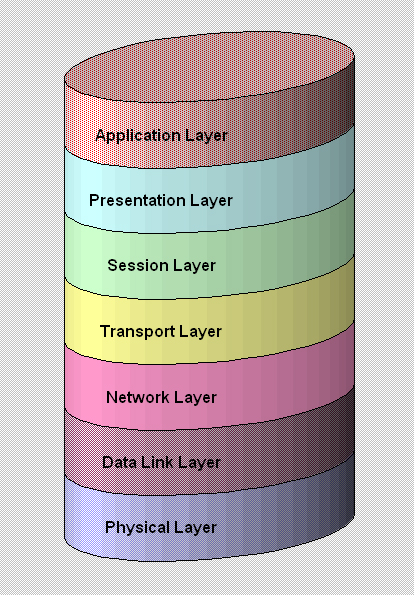
\includegraphics[width=0.5\textwidth]{Grafiken/osi_modell.jpg}
\caption{Das \osi im Überblick \cite{osi_modell}}
\label{osi_modell}
\end{figure} 
Diese Grafik stellt die Schichten des \osi da. Das \osi, (Open Systems Interconnection Model) ist ein allgemeines Kommunikationsmodell,  das die Kommunikation unterschiedlichster Geräte ermöglicht. Es beschreibt ein komplettes Telekommunikationsnetzwerk. Die einzelnen Funktionen sind in 7 Schichten aufgeteilt. 

Das \osi standardisiert die Netzwerk Architektur. Dadurch können Hersteller Lösungen anbieten, die auf der ganzen Welt genutzt werden können. Eine proprietäre Lösung hätte zu Insellösungen geführt. Ein weiterer Vorteil ist, dass die einzelnen Schichten, oder Layer, über Schnittstellen miteinander kommunizieren. Das ermöglicht ein Austauschen einzelner Komponenten, ohne die gesamte Architektur ändern zu müssen.

Da das \osi nur ein Referenzmodell darstellt, müssen die einzelnen Schichten konkret implementiert werden. Diese Implementierungen sind eigene Protokolle. 

\subsection{Der Layer 2}
Der Layer 2, Data Link Layer, setzt auf dem Physical Layer auf und stellt dem Network Layer seine Dienste zur Verfügung. Der Physical Layer beschriebt das Medium über das die Signale übertragen werden. Hier findet noch keine Logik statt. 

Die Aufgaben des Layer 2 im Überblick:
\begin{itemize}
	\item Aufteilung in Pakete
	\item Fehlerkontrolle
\end{itemize} 

\subsubsection{Aufteilung in Frames}
Die Datenblöcke werden im Layer 2 in Frames aufgeteilt. Die Vorteile des Framing sind die schnellere Nutzung eines shared Mediums und dass fehlerhafte Daten nicht komplett übertragen werden müssen.
\subsubsection{Fehlerkontrolle}
Der Data Link Layer führt eine Fehlerkontrolle durch. Dazu zählen eine Suche nach Duplikaten, nach inkorrekt oder unvollständig gesendeten Paketen. Wenn ein Fehler entdeckt wird, wird eine neue Übertragung der Frames angefordert \cite[S. 91]{SWB-107223570}. Die Fehlerkontrolle wird über den \glqq Cyclic Redundancy Check\grqq ~CRC durchgeführt. Dieses Verfahren ist eine Möglichkeit zur Prüfsummenberechnung, die beim Sender und der Senke durchgeführt wird. Sind beide Prüfsummen gleich, kann angenommen werden, dass das Frame korrekt übertragen wurde. 

Die Frames werden mit Sequence Numbers durchnummeriert. Der Empfänger prüft, ob die Frames in der richtigen Reihenfolge ankommen. Bei einer \glqq out-of-sequence transmission\grqq ~kann von einem verlorenen Frame ausgegangen werden, das entsprechende Frame wird neu angefordert, bzw. Layer 3 wird benachrichtigt.
\section{Die Layer 2 Protokolle im Überblick}

\subsection{Ethernet}
Ethernet ist ein weit verbreitetes Layer 2 Protokoll. 90\% aller lokal installierten Netzwerke sind mit Ethernet realisiert\cite{SWB-097965316}. Ethernet wurde ursprünglich für die Anbindung eines Druckers bei der Firma Xerox Corporation entwickelt. Die damalige Übertragungsgeschwindigkeit von 2,94 Mbit/s wurde auf aktuell 100 Gbit/s gesteigert, weitere Steigerungen sind zu erwarten.

Die Daten werden im Ethernet über einen eigenen Übertragungskanal transportiert. Kollisionen werden durch \glqq CSMA/CD\grqq ~entdeckt, bzw. aufgelöst. Die Übertragung läuft gleichberechtigt und verbindungslos. Die Daten werden an alle Teilnehmer weitergeleitet, diese vergleichen die Empfängeradresse mit ihrer eigenen und verwerfen die Frames, die nicht an sie adressiert sind. Diese Aussage kann eingeschränkt werden, da Switche die Daten nur an Ports leiten, an denen die entsprechenden Senken angeschlossen sind. 

\subsubsection{Gebräuchliche Übertragungsmedien des Ethernet}
\begin{figure}[H]
\begin{minipage}[hbt]{.28\linewidth}
	\centering
	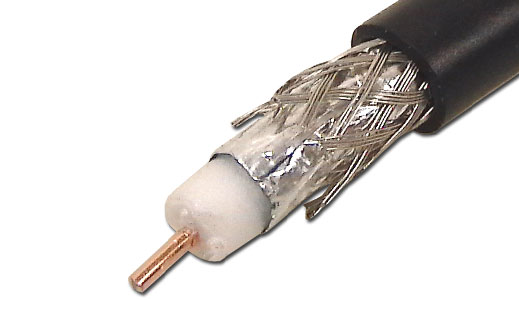
\includegraphics[width=0.9\linewidth]{Grafiken/koaxkabel.png}
	\caption{Koaxkabel \cite{koax_kabel}}
	\label{koaxkabel}
\end{minipage}
\hfill
\begin{minipage}[hbt]{.28\linewidth}
	\centering
	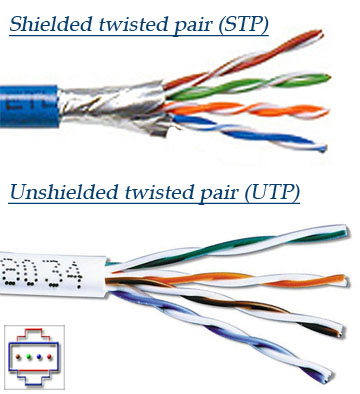
\includegraphics[width=0.9\linewidth]{Grafiken/twistetPair.jpg}
	\caption{Twistet Pair Kabel \cite{tw_kabel}}
	\label{twkabel}
\end{minipage}
\hfill
\begin{minipage}[hbt]{.28\linewidth}
	\centering
	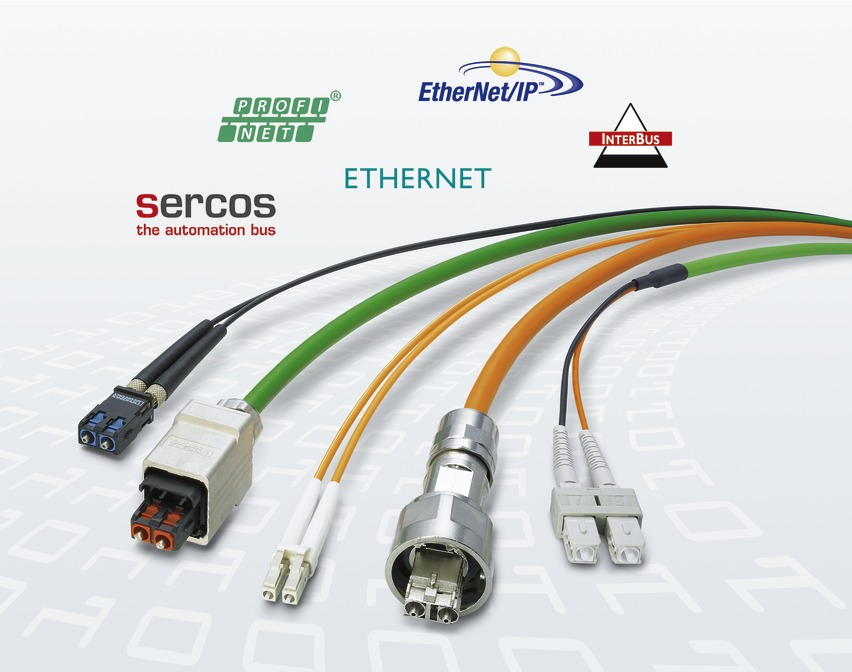
\includegraphics[width=0.9\linewidth]{Grafiken/lwl_leiter.jpg}
	\caption{Lichtwellenleiter \cite{lwl_leiter}}
	\label{lwlleiter}
\end{minipage}
\end{figure}
 
Historisch gesehen muss das Koaxialkabel als Medium des Ethernet genannt werden. Das Koaxkabel wurde 1990 mit der Einführung von 10BaseT (IEEE 802.3i) durch Unshielded Twisted Pair Kabel ersetzt. Ab 1998 wurden mit der Einführung des Gigabit Ethernet auch Lichtwellenleiter genutzt. 

\subsubsection{Zugriff auf das Medium}
Historisch gesehen nutzt Ethernet das Übertragungsmedium als Shared Medium. Die einzelnen Teilnehmer wurden am selben Koaxialkabel über T-Stücke angeschlossen. Um Kollisionen zu vermeiden, wurde ein geeignetes Verfahren zur Vermeidung benötigt. Von einer Kollision spricht man, wenn mehrere Teilnehmer gleichzeitig auf das Medium zugreifen würden, also Signale aussenden. Die Signale würden sich gegenseitig überlagern und wären nicht mehr nutzbar. Bei Ethernet wird CSMA/CD eingesetzt. Bei diesem Verfahren wird vor dem Senden geprüft, ob die Leitung frei ist. Erst wenn die Leitung frei ist wird gesendet (Carrier Sense). Wenn zufällig mehrere Teilnehmer gleichzeitig ein Signal aussenden (Multiple Access) kommt es dennoch zu Kollisionen. Der/Die Sender prüfen während dem Senden, ob es zu Kollisionen kommt (Collision Detect) und brechen ihre Übertragung im Fall einer Kollision ab. Nach einem Abbruch wird eine zufällige Zeit gewartet bis erneut gesendet wird. Der Grund, warum es trotz diesem Verfahren zu Kollisionen kommen kann, ist die Signallaufzeit. Die Signale brauchen eine gewisse Zeit um über die Leitungen übertragen zu werden. 

In seinen Anfangszeiten übertrug Ethernet im Halbduplex Verfahren. Das bedeutet, dass ein Übertragungskanal zum Senden und zum Empfangen genutzt wird. Dadurch halbiert sich natürlich im schlimmsten Fall die Datenrate. Mit der Einführung von Twisted Pair Kabeln und Lichwellenleitern wurde Ethernet auf den Vollduplex Betrieb umgestellt. Dadurch konnte die Übertragungsrate gesteigert werden und Kollisionen wurden unwahrscheinlicher.
\begin{figure}[H]
	\centering
	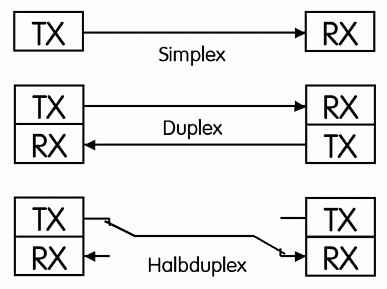
\includegraphics[width=0.4\linewidth]{Grafiken/duplex.jpg}
	\caption{Unterschied der Duplex Übertragungen \cite{duplex}}
	\label{duplex}
\end{figure}
 
 \subsubsection{Frames}
Um Daten über Ethernet übertragen zu können werden sie in Frames aufgeteilt. Der Vorteil daran ist, dass ein Sender bei großen Übertragungen nicht das gesamte Netzwerk belegt und dass bei einer fehlerhaften Übertragung nur einzelne Frames neu versandt werden müssen. Der Ausdruck Frame kann wörtlich genommen werden. Die Nutzdaten werden in einen Rahmen (Frame) eingepackt.

Neben den eigentlichen Nutzdaten enthält ein Frame:
\begin{itemize}
	\item Die Präambel (dient u.a. zur Synchronisation der Empfängerstationen) 
	\item Die Hardware Quell- und Zieladresse
	\item Ein Typ- oder Längenfeld
	\item Eine Checksumme
\end{itemize}
\begin{figure}[H]
	\centering
	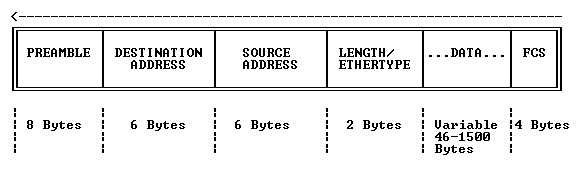
\includegraphics[width=0.9\linewidth]{Grafiken/ethernet_frame.jpg}
	\caption{Ethernet 802.3 Frame \cite{ethernet_frame}}
	\label{ethernet_frame}
\end{figure}

Die Präambel enthält eine Bitfolge, die dem Empfänger signalisiert, dass ein Rahmen ankommt. Die Präambel besteht aus 8 Bytes mit einer alternierenden Folge aus 0 und 1. Die letzten 2 Bits im letzten Byte sind immer 1. Hier besteht ein kleiner Unterschied zwischen DIX und IEEE. Obwohl die Bitfolgen die gleichen sind, ist die Präambel im IEEE Standard formell in die 7 Byte lange Präambel und den 1 Byte langen Start-of-Frame-Delimiter aufgeteilt.
 
Die Adressen sind MAC Adressen. Dieser werden von der IEEE an die Hersteller von Ethernet Komponenten vergeben und müssen weltweit eindeutig sein.

\subsubsection{Topologie}
Ethernet ist keiner bestimmten Netzwerk Topologie zuzuordnen. Heute gebräuchlich ist eine Sterntopologie, andere Formen sind aber auch möglich.   


\subsection{LAPD}
\blindtext

\subsection{PPP}
Router - Router und Host - Netzwork Verbindungen über synchrone und asynchrone Kreise. Enthält ein Protokoll Feld um das Network Layer Protokoll zu Identifizieren \cite[S. 102]{SWB-107223570}  

Während in einzelnen Gebäuden meist LANS zum Einsatz kommen, werden für die weitreichende Verbindungen meist Punkt-zu-Punkt-Standleitungen eingesetzt. Diese Leitungen verbinden weit entfernte Router miteinander, hinter denen LANS mit mehren Hosts wie Personal-Computer, Workstation oder Server angeschlossen sind. Die Verbindung in die Außenwelt von diesen LANS aus, wird eben genau über diese Router laufen. Und hier kommt das PPP (Point-to-Point Protocol) zum Einsatz.

PPP ist in RFC 1661 definiert und wurde in mehreren anderen RFCs weiter ausgearbeitet wie in RFC 1662 und 1663.




\section{Bedeutungen der Protokolle im \osi }

%indirekte Quellen einbinden
\nocite{*} 

%Quellenangabe auf eigener Seite
\newpage
\sloppy
\printbibliography 



%Abbildungsverzeichnis auf eigener Seite
\newpage
\listoffigures

\end{document}